\documentclass[titlepage,oneside,final,14pt]{extarticle} % тип документа (титульник, односторонняя, финальная версия, 14 пункт по дефолту)

\usepackage[utf8]{inputenc} % кодировка
\usepackage[english,russian]{babel} % переносы и поддержка языка
\usepackage{indentfirst} % отступы в абзаце
\usepackage{vmargin}
\usepackage{hyperref} % гиперссылки
\usepackage{listings} % листинги кода
\usepackage{color} % создание цветов
\usepackage{graphicx} % картинки
\usepackage{tempora} % шрифт
\usepackage{float} % чтоб картинки не плавали [H]
\usepackage{setspace} 
\usepackage{chngcntr} 
\usepackage{ccaption} 
\usepackage{titlesec} % для заголовков
\usepackage{ragged2e} % для выравнивания по ширине
\usepackage{enumitem} % для межстрочного интервала в списках

\setlist{noitemsep} % убирает отступы для элементов списка
\titleformat{\section}[hang]{\normalfont\Large\bfseries\filcenter}{\thesection}{1em}{}[] % настройки заголовков
\titleformat{\subsection}[hang]{\filcenter\bfseries}{\thesubsection}{1em}{}[]
\titleformat{\subsubsection}[hang]{\filcenter\bfseries}{\thesubsubsection}{1em}{}[]
\newcommand{\sectionbreak}{\clearpage} % для разрыва листа для новой секции

\RequirePackage{caption}
\DeclareCaptionLabelSeparator{defis}{ --- }
\captionsetup{justification=centering,labelsep=defis} % для тире в подписях к картинкам

\counterwithin{figure}{section} % счетчик для картинок
\onehalfspacing % полуторный интервал
\graphicspath{{./images/}} % путь к папке с картинками
\setpapersize{A4} % а4 лист
\setmarginsrb{30mm}{20mm}{15mm}{20mm}{0pt}{0mm}{0pt}{10mm} % поля - левое, верхнее, правое, нижнее
\parindent=1.25cm % абзацный отступ
\sloppy % чтоб не вылезало за пределы листа
\lstset{language=Java,
	showspaces=false,
	showtabs=false,
	breaklines=true,
	showstringspaces=false,
	breakatwhitespace=true,
	commentstyle=\color{pgreen},
	keywordstyle=\color{pblue},
	stringstyle=\color{pred},
	basicstyle=\linespread{1}\small\ttfamily,
	columns=fullflexible
} % настройки листинга кода

\definecolor{pblue}{rgb}{0.13,0.13,1}
\definecolor{pgreen}{rgb}{0,0.5,0}
\definecolor{pred}{rgb}{0.9,0,0}
\definecolor{pgrey}{rgb}{0.46,0.45,0.48}

\hyphenpenalty=10000 % для отсутствия переносов
\justifying % по ширине

\author{Bulychev Ivan}
\title{Лабораторная работа №1}

\begin{document}
	
\begin{titlepage}
	\begin{spacing}{1.1}
		\begin{center}		
			ФЕДЕРАЛЬНОЕ АГЕНТСТВО СВЯЗИ 
			\\
			Федеральное государственное бюджетное образовательное учреждение высшего образования
			\\
			<<ПОВОЛЖСКИЙ ГОСУДАРСТВЕННЫЙ УНИВЕРСИТЕТ ТЕЛЕКОММУНИКАЦИЙ И ИНФОРМАТИКИ>>
			\\			
			\vspace{1em}
			Факультет информационных систем и технологий
			\\
			Кафедра программного обеспечения и управления в технических системах
			\\
			\vspace{7em}
			\bfseries\Large
			ОТЧЕТ
			\\
			ПО ЛАБОРАТОРНОЙ РАБОТЕ № \underline{\hspace{0.4em}1\hspace{0.4em}}
			\\
			\vspace{0.5em}
			\normalfont
			\normalsize
			по дисциплине
			\underline{\hspace{4em}Параллельное программирование\hspace{4em}}
			\\
			\small
			\hspace{4em} название (при наличии)
			\normalsize
			\\
			\hspace{3em}			
			\underline{\hspace{3em}Запуск консольного приложения на кластере MPI\hspace{3em}}
			\\
			\small
			\hspace{4em} название работы (при наличии)
			\normalsize
			\\		
	\end{center}			
			\vspace{5em}
			\begin{minipage}{0.5\textwidth}
				\begin{flushleft}					
				\end{flushleft}
			\end{minipage}
			\begin{minipage}{0.5\textwidth}
				\begin{center}
					\bfseries
					ВЫПОЛНИЛ
					\\
					\normalfont
					студент \hspace{1ex} \underline{гр. ПО--61} \hspace{1ex} \underline{Булычев И. Д.}
					\\
					\small
					\hspace{3.5em} (группа) \hspace{3.5em} (ФИО)
					\normalsize\bfseries
					ПРОВЕРИЛА
					\\
					\normalfont
					\hspace{1ex} \underline{к. т. н., доцент} \hspace{1ex} \underline{Мезенцева Е. М.}
					\\
					\small
					(должность) \hspace{5em} (ФИО)
					\\	
					\normalfont				
				\end{center}
			\end{minipage}
		\begin{center}
			\vspace{6em}
			Самара
			\\
			2019
			\end{center}

			

\end{spacing}
\end{titlepage}
\setcounter{page}{2}
%\input{title.tex}

\section{Цель лабораторной работы}

\subsection{Цель работы}

Разработать и запустить на кластере программу на любом из языков программирования, поддерживающий работу с библиотекой MPI.

\subsection{Задачи}

\begin{enumerate}
	\item Установить средства работы с MPI, настроить кластер;
	\item Разработать программу с использованием библиотеки MPI	(каждый процесс в кластере должен вывести на экран свой номер, общее число процессов, имя хоста, на котором он выполняется, время выполнения параллельной части программы);
	\item Выполнить запуск программы на собранном кластере.
\end{enumerate}

\subsection{Используемое программное обеспечение}

Для выполнения лабораторной работы мною было использовано следующее программное обеспечение:
\begin{itemize}
	\item ОС Ubuntu 18.10
	\item IDE Intellij Idea 2018.3
	\item JDK 1.8
	\item MPJ Express 0.44
\end{itemize}

\section{Ход выполнения лабораторной работы}

\subsection{Установка библиотеки MPJ Express}

Для выполнения лабораторной работы необходимо установить библиотеку MPJ Express~--- технология MPI для языка программирования Java.
Для этого нужно перейти на сайт \href{http://mpj-express.org/}{http://mpj-express.org/}, перейти в раздел \href{http://mpj-express.org/download.php}{Download}, выбрать ссылку \href{https://sourceforge.net/projects/mpjexpress/files/releases/}{MPJ Express Software} и, в зависимости от операционной системы, выбрать архив с нужным расширением (.zip --- для ОС Windows, .tar.gz --- для ОС Linux) и версией.

После загрузки архива нужно его распаковать (я распаковал в папку /home/dstrmv/mpj/), и установить переменные среды MPJ\_HOME (путь до директории распаковки --- в моем случае это /home/dstrmv/mpj/) и PATH (путь до папки bin --- /home/dstrmv/mpj/bin).

Установка переменных среды для ОС Linux выполняется командами:
\begin{itemize}
	\ttfamily
	\item export MPJ\_HOME=path/to/mpj/
	\item export PATH=\$MPJ\_HOME/bin:\$PATH
	\normalfont	
\end{itemize}

\subsection{Настройка Intellij Idea для работы с MPJ Express}

\subsubsection{Добавление библиотеки в classpath}

После создания проекта, нужно перейти в настройки проекта (File -- Project Structure), выбрать вкладку Libraries, нажать на +, выбрать Java, и указать путь до библиотеки lib/mpj.jar. Название библиотеки появится в списке.

\begin{figure}[H]
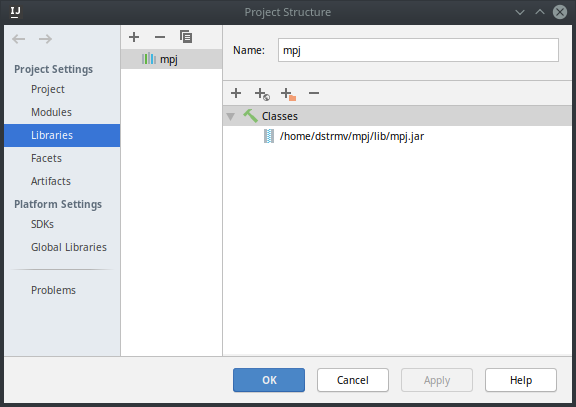
\includegraphics[width=0.9\linewidth]{project_structure.png}
\centering
\caption{Окно <<Project Structure>>}
\end{figure}


\subsubsection{Настройка параметров компиляции}

После добавления библиотеки, нужно создать нужную конфигурацию запуска приложения. Для этого нужно в меню Run выбрать пункт <<Edit configurations...>>, и в появившемся окне в поле <<VM options>> добавить строчку <<\ttfamily-jar~\$MPJ\_HOME\$/lib/starter.jar~-np~2\normalfont>> (здесь первым параметром указывается библиотека для запуска MPI приложения, а вторым --- количество процессов выполняемой программы). Также можно добавить переменную окружения MPJ\_HOME в поле <<Environment variables>>.

\begin{figure}[H]
	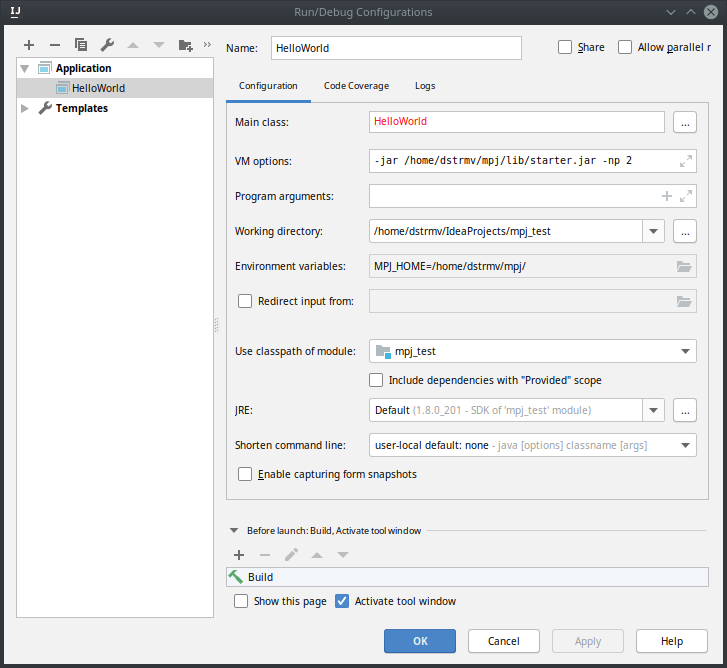
\includegraphics[width=0.9\linewidth]{edit_configurations.png}
	\centering
	\caption{Окно <<Run/Debug Configurations>>}
\end{figure}

\section{Результаты выполнения лабораторной работы}

\subsection{Листинг приложения}

\begin{lstlisting}
import mpi.*;

public class HelloWorld {
    public static void main(String[] args) {

        int rank, size, resultlen;
        double startwtime = 0.0, endwtime;
        String name;

        MPI.Init(args); // MPI initialization
        startwtime = MPI.Wtime(); // system time
        size = MPI.COMM_WORLD.Size(); // total amount of processes
        rank = MPI.COMM_WORLD.Rank(); // process's number
        name = MPI.Get_processor_name(); // pc name
        endwtime = MPI.Wtime();
        System.out.printf("Hello world from process %d of %d at %s as %f second \n",
        rank, size, name, endwtime-startwtime);
        MPI.Finalize(); // finish parallel part of program
    }
}

\end{lstlisting}

\subsection{Результат выполнения}


\ttfamily
\noindent
MPJ Express (0.44) is started in the multicore configuration

\noindent
Hello world from process 0 of 2 at dstrmv-pc as 0,000000 second
 
\noindent
Hello world from process 1 of 2 at dstrmv-pc as 0,000000 second 

\normalfont

\begin{figure}[H]
	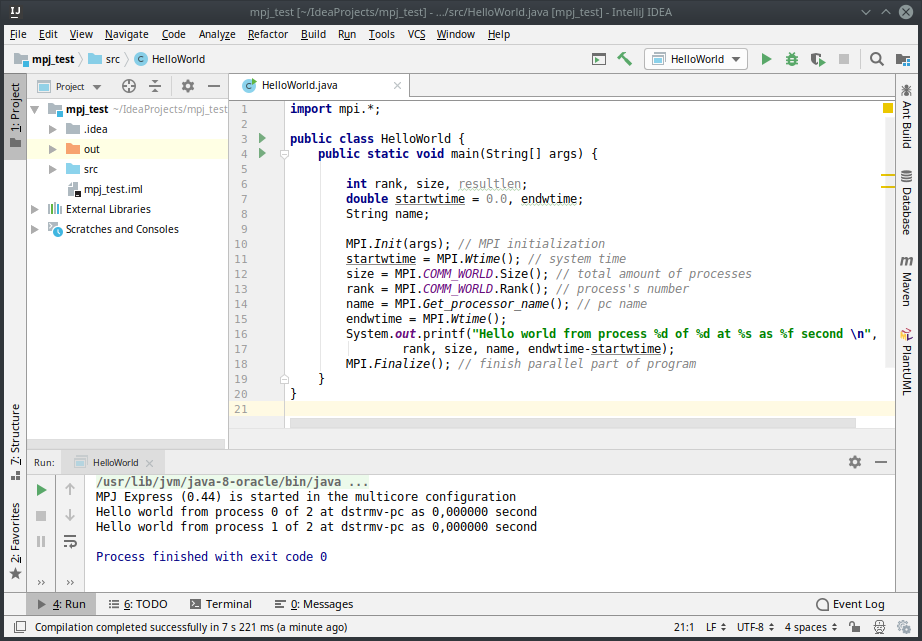
\includegraphics[width=0.9\linewidth]{code_listing_results}
	\centering
	\caption{Листинг и результат выполнения}
\end{figure}

\section{Выводы по результатам выполнения лабораторной работы}

В ходе работы была написано консольное приложение на языке Java в среде программирования Intellij Idea, к которой подключена библиотека MPJ Express. Каждый процесс
выводит на экран фразу Hello world from process, далее выводится номер
данного процесса, фраза of, после которой подставляется общее число
процессов, фраза at, после которой вставляется имя хоста, на котором
выполняется данный процесс, фраза as, после которой подставляется время выполнения процедур MPI\_Comm\_size, MPI\_Comm\_rank, MPI\_Get\_processor\_name.

Выполнен тестовый запуск программы на кластере, состоящем из ядер процессора компьютера.

\end{document}
